\chapter{Design Methodology}
\label{chap:design_methodology}

This project follows a design, build, and test approach, with the primary objective of designing, manufacturing, and demonstrating a cost-effective rotary climbing wall at full scale.

The project employs a modified design process based on the methodology presented by \cite{dieter_schmidt_2021}. This process is divided into two phases: conceptual design and detailed design.

\section{Phase I: Conceptual Design}

\subsection{Identification of Customer Needs}
The first phase begins with identifying and gathering customer requirements to ensure that the design aligns with the expectations and functional needs of the users. A thorough exploration of customer needs is provided in Chapter \ref{chap:climbing_performance}.

\subsection{Problem Definition}
A clear problem statement is formulated based on the identified customer needs, serving as the foundation for the design process. Details can be found in Section \ref{sec:problem_definition}.

\subsection{Gathering Information}
Relevant information is collected from technical articles, patents, and design journals to support the generation of potential design concepts. Chapter \ref{chap:technology_review} presents an analysis of various market products that address the problem, and from these, key engineering and design parameters are derived.

\subsection{Concept Generation}
Using brainstorming techniques and creative design methods, multiple design concepts are generated. These concepts are detailed in Chapter \ref{chap:concept_design}.

\subsection{Evaluation of Concepts}
The generated concepts are evaluated based on key selection criteria, including feasibility, cost, and performance.

\subsection{Concept Integration}
The most suitable concept is selected and further refined for integration into a comprehensive system design.

\subsection{Design Review}
The final concept undergoes a rigorous design review to ensure all requirements and specifications are met before transitioning to the detailed design phase.

\section{Phase II: Detail Design}

\subsection{Design Verification}
In this phase, each aspect of the design is verified through structural and performance analysis, including calculations and Finite Element Method (FEM) simulations.

\subsection{Detailed Engineering Drawings}
Detailed engineering drawings are produced, specifying dimensions, tolerances, and materials, ensuring the design is ready for manufacturing.

\begin{figure}[H]
    \centering
    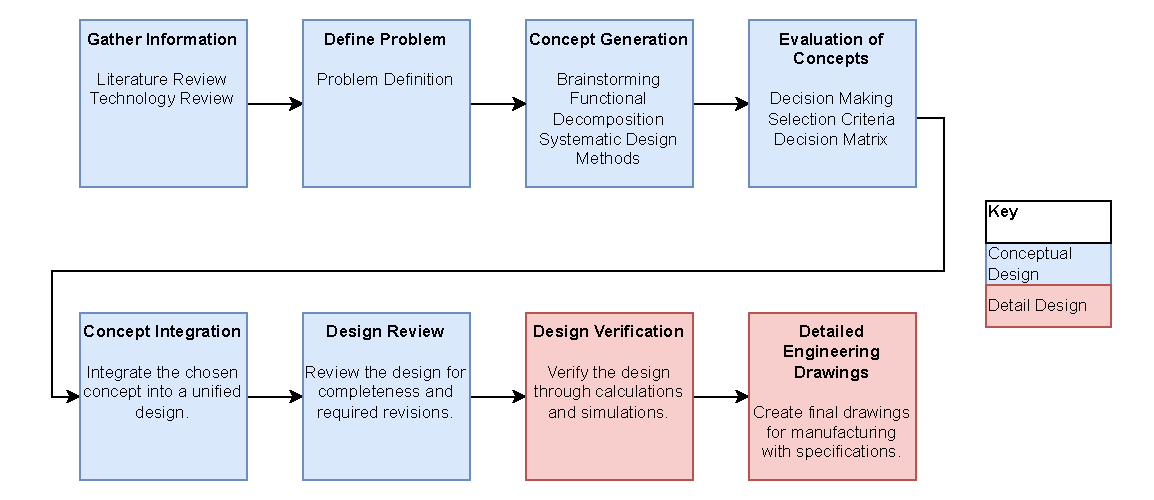
\includegraphics[width=1\textwidth]{figs/DesignMethodologyFlow.pdf} % Path to your PDF
    \caption{Flowchart depicting the design process followed in the project.}
    \label{fig:design_process_flowchart}
\end{figure}


